\section{approach}
\label{sec:approach}
In this section, we first formulate the just-in-time defect prediction and provide an overview of our framework. We then describe the details of each part inside the framework. Finally, we present an algorithm for learning effective settings of our model's parameters. 
\subsection{Framework Overview}
\label{sec:overview}

\begin{figure}
\center
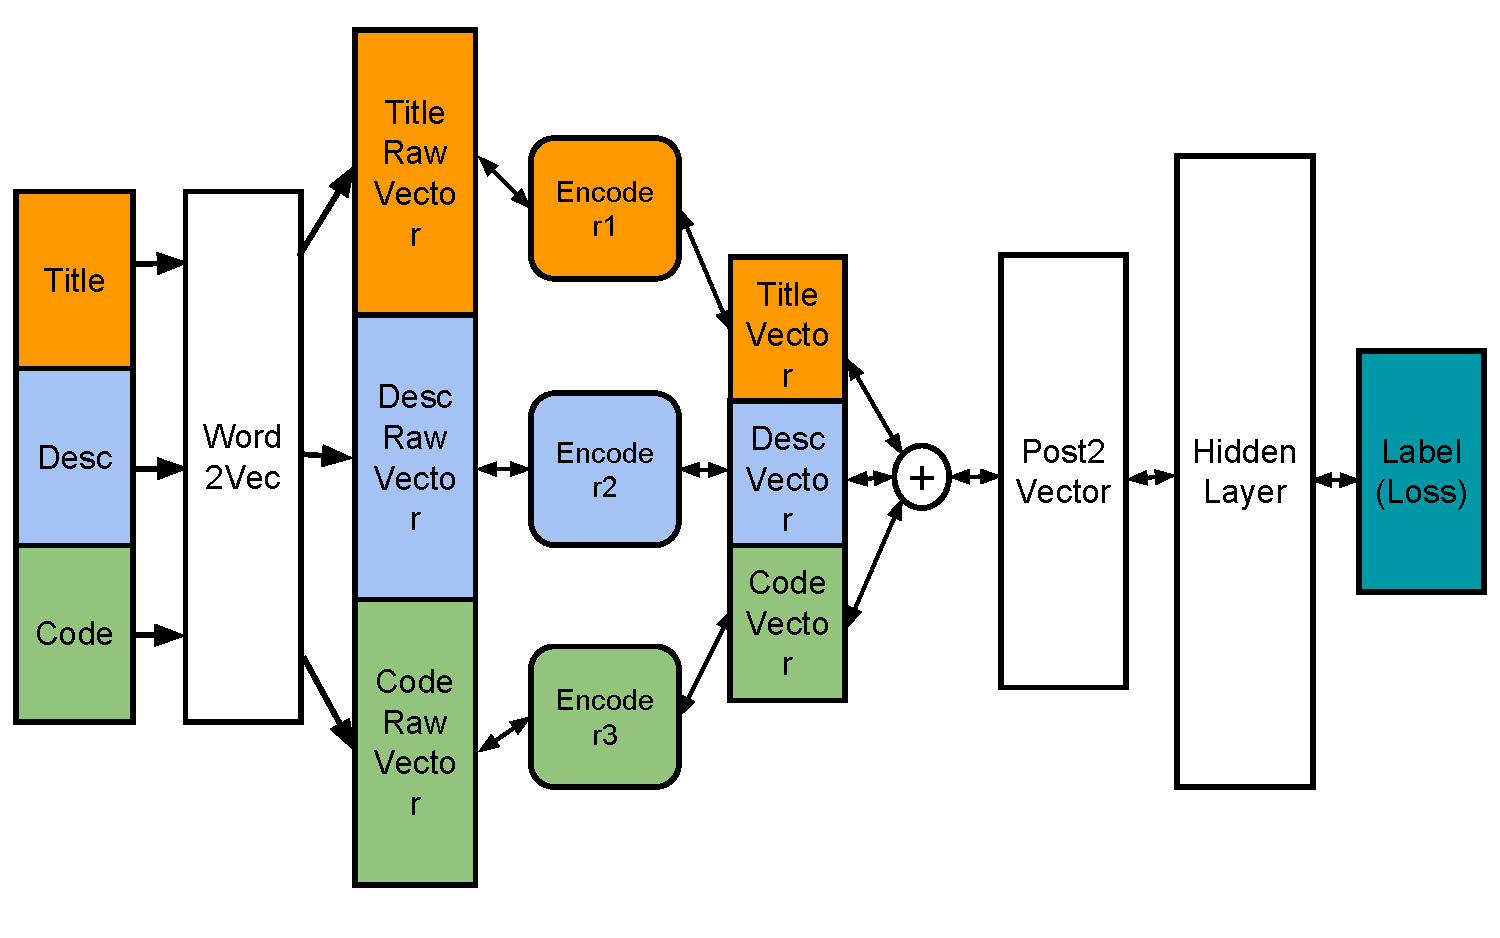
\includegraphics[scale=0.36]{figs/framework.pdf}
\caption{Architecture of our \textit{commit message module} used to build an embedding vector from a commit message.}
\label{fig:msg_model}
\vspace{-0.4cm}
\end{figure}

